\documentclass{article}

\author{Pedro Henrique Limeira da Cruz}
\title{Resistência dos Materiais - II}

\usepackage[margin=0.8in]{geometry}
\usepackage{indentfirst}
\usepackage{fancyhdr}
\usepackage{tcolorbox} 
\usepackage{graphicx}
\usepackage{amsmath}
\usepackage{amssymb}
\usepackage{enumitem}
\usepackage{tabularx} % in the preamble
\usepackage{wrapfig}
\usepackage{subcaption}
\usepackage{caption}

% Create a Todo list
\newlist{todolist}{itemize}{2}
\setlist[todolist]{label=$\square$}

% Fix vspace inside wrapfigure
\setlength\intextsep{0pt}


\newcolumntype{Y}{>{\centering\arraybackslash}X}

% Create a new command to be used in the align environment in multiple line equations do only the last equation is numbered  
\newcommand{\n}{\nonumber \\ }
\makeatletter
\let\inserttitle\@title
\makeatother
% Set the style of the page 
\pagestyle{fancy}
\fancyhf{}
\rhead{Pedro Henrique L. da Cruz}
\lhead{\inserttitle}
\rfoot{Page \thepage}

\usepackage{hyperref}
\hypersetup{
    colorlinks=true,
    linkcolor=black,
    filecolor=magenta,
    urlcolor=cyan,
}

% Begin the Document 
\begin{document}

\maketitle
\thispagestyle{empty}

% Add the image inside a figure in as the first page
% \begin{figure}[h]
%     \begin{center}
%         
\includegraphics[scale = 0.15]{/Users/pedrocruz/Documents/UNICAMP/ES101/ES101 - Robotic Arm/img/unicamp.png}
%     \end{center}
% \end{figure}

% Change to the Next page 
\newpage
\tableofcontents
\newpage

\section{Tensão de Cisalhamento em Vigas}
\subsection{Vigas de Seção Transversal Regular}

\subsubsection{Introdução}
\begin{wrapfigure}{r}{0.3\textwidth}
\vspace{-15px}
\centering
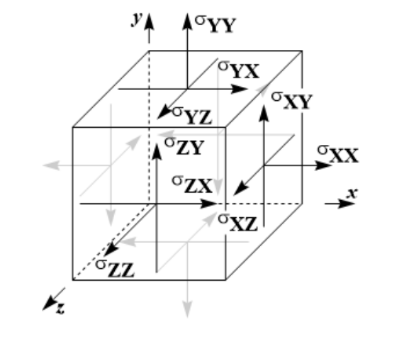
\includegraphics[width=.25\textwidth]{imgs/tensões.png}
\vspace{-15px}
\caption{Tensões em um Ponto}
\label{img:tensions}
\end{wrapfigure}
Em resistência dos Materiais I, vimos que cada ponto de um corpo possui possui tensões que estão sendo aplicadas nele, como podemos ver na figura \ref{img:tensions}. Além disso, vimos em Resmat I como calcular as tensões Normais ($\sigma_{XX}$) na face de uma viga, e não somente em um ponto.

Nosso objetivo de estudos nesse capitulo, entretanto, é conseguir calcular as tensões de \textbf{cisalhamento} (que chamaremos de $\tau$) sobre toda a área de uma viga. Na imagem supracitada, as tensões de Cisalhamento são as que possuem os índices diferentes (\emph{e.g} $\sigma _{XZ}$).

$\\$

\subsubsection{Análise de Esforços Internos}
\begin{wrapfigure}{l}{.3\textwidth}
    \centering
    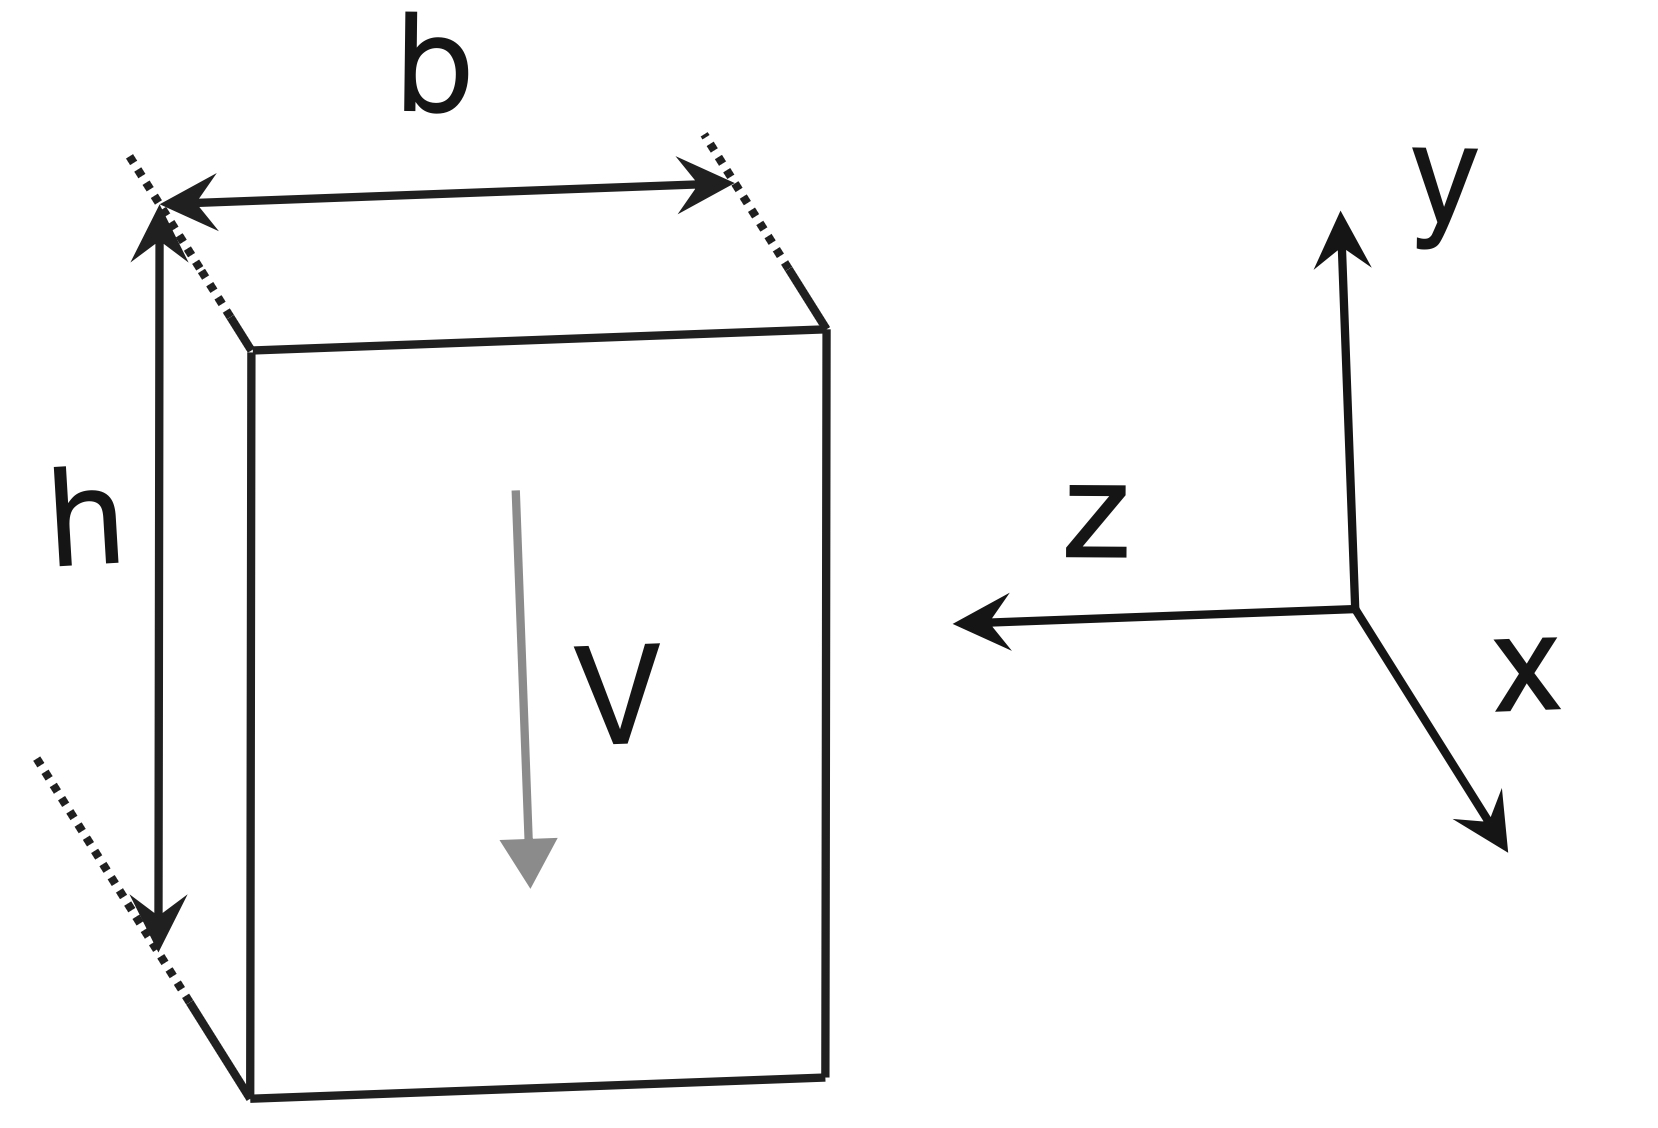
\includegraphics[width=.3\textwidth]{imgs/IMG_0278.jpeg}
    \caption{Caption}
    \label{img:viga_tensão}
\end{wrapfigure}

Considerando uma viga de seção transversal submetida a um esforço conrtante positivo ($V$, também chamado de Força Cisalhante) como visto na imagem, e considerando também:
\begin{itemize}
    \item As tensões de Cisalhamento $\tau$ agindo sobre a seçaõ transversal são paralelas ao esforço cortante.
    \item As tensões de Cisalhamento são uniformemente distribuídas ao longo da largura da viga.
\end{itemize}

Somos capazes de determinar a intensidade da tensão de cisalhamento em qualquer ponto da seção transversal. 

Para começar nossas análises, vamos entender melhor quais são as tensões de cisalhamento que atuam sobre um elemento infinitesimal.

Considerando o \textbf{elemento infinitesimal}, mostrado na figura \ref{fig:elemento_infinitesimal}, podemos observar que, \textbf{para toda tensão agindo em um plano, há outra, de mesma intensidade, agindo em uma face perpendicular} (e.g como há um esforço cortante para baixo, também há uma tensão de cisalhamento para baixo. Devido ao que foi dito, também haverá uma tensão na face superior desse elemento infinitesimal).

Além disso, devido ao equilíbrio estático da peça inteiera (e por conseguinte do element infinitesimal) temos a presença de duas outras tensões de cisalhamento, para compensar a para baixo haverá uma para cima, e para compensar a desenvolvida perpendicularmente teremos outra para o lado, resultando em uma distribuição como vista na figura \ref{fig:elemento_infinitesimal}.

\begin{figure}[h]
    \centering
    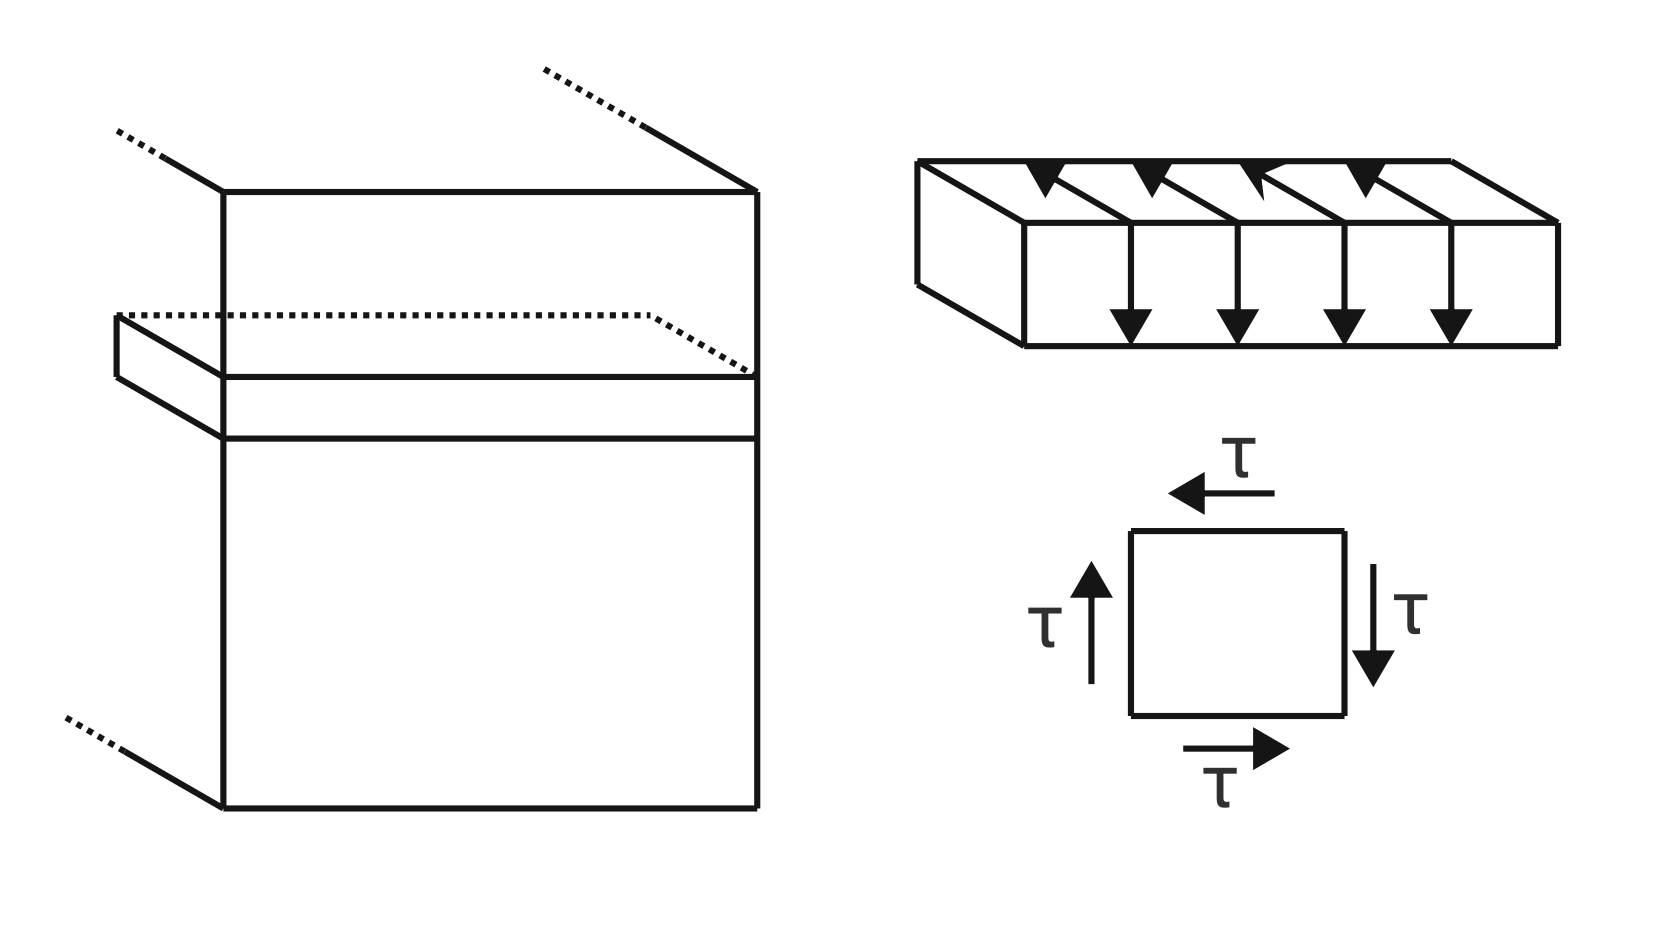
\includegraphics[width=.3\textwidth]{imgs/IMG_0303.jpeg}
    \caption{Caption}
    \label{fig:elemento_infinitesimal}
\end{figure}

Temos então que se há uma tensão de cisalhamento para baixo em uma face, também haverá uma tensão na face perpendicular. Para o caso de uma viga onde, na sua face superior e inferior não haja um carregamento, isso implica que não haverá uma tensão para baixo e, por conseguinte, não haverá uma tensão de cisalhamento na horizontal. Descrevendo matematicamente temos:
\begin{align}
    \tau = 0 \ \, y =\pm h/2
\end{align}

Tendo como início do nosso sistema de coordenadas o meio da viga.
\subsubsection{Derivação da Fórmula de Tensão de Cisalhamento}
Anteriormente analisamos o comportamento geral, e a localização, das tensões de cisalhamento em uma viga. Vimos, tabém, que ha tensões de cisalhamento tanto na horizontal quanto na vertical, sendo que, na engenharia e para o projeto de vigas, o que mais importa são as tensões verticais. 

As tensões Verticais, entretanto, são muito mais complexas de seres determinadas do que as horizontais. Isso, entretanto, não é um problema, pois no capítulo anterior acabos de ver que as tensões verticais e horizontais possuem o mesmo valor em módulo, com isso, iremos ver como se calcula as tenões de cisalhamento.

Iremos, a seguir, ver uma forma de calcularmos os valores das tensões cisalhantes a partir dos carregamentos externos, das tensões normais (que vimos como fazer em resmat I) e do equilíbrio estático.

Considerando uma viga submetida a uma flexão não uniforme, como mostrado abaixo:

\begin{figure}[h]

    \centering
    \begin{subfigure}[t]{.45\textwidth}
        \centering
        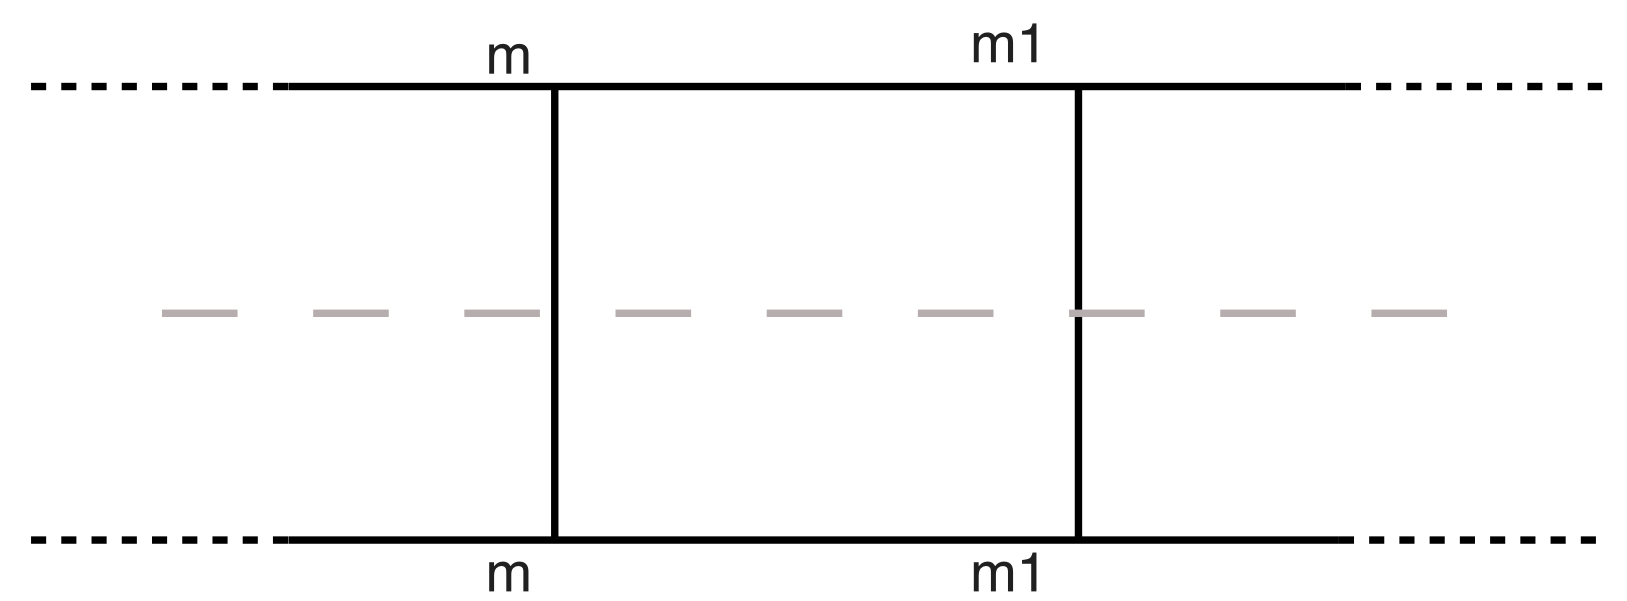
\includegraphics[width=\textwidth]{imgs/IMG_0298.jpeg}
        \caption{Viga}
        \label{fig:enter-label}
    \end{subfigure}
    \begin{subfigure}[t]{0.45\textwidth}
        \centering
        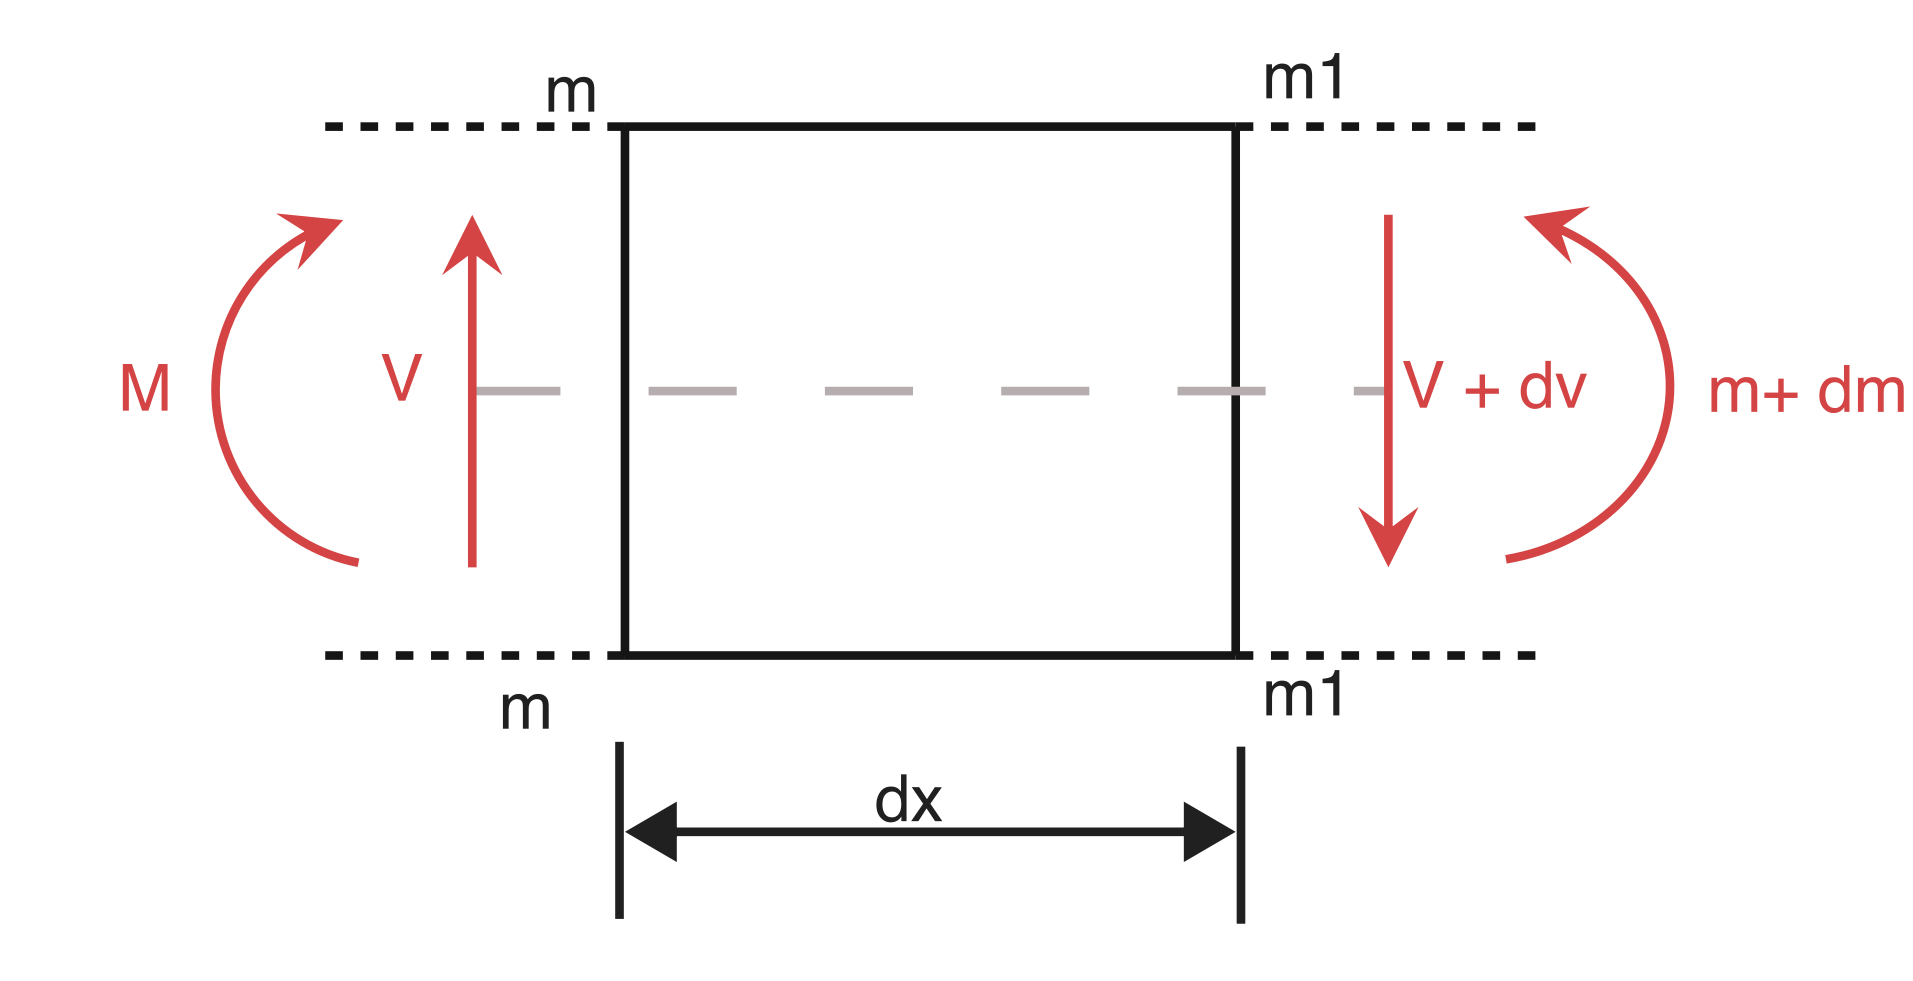
\includegraphics[width=.8\textwidth]{imgs/IMG_0299.jpeg}
        \caption{Carregamento Não uniforme}
        \label{fig:enter-label}
    \end{subfigure}
        \begin{subfigure}[t]{.45\textwidth}
        \centering
        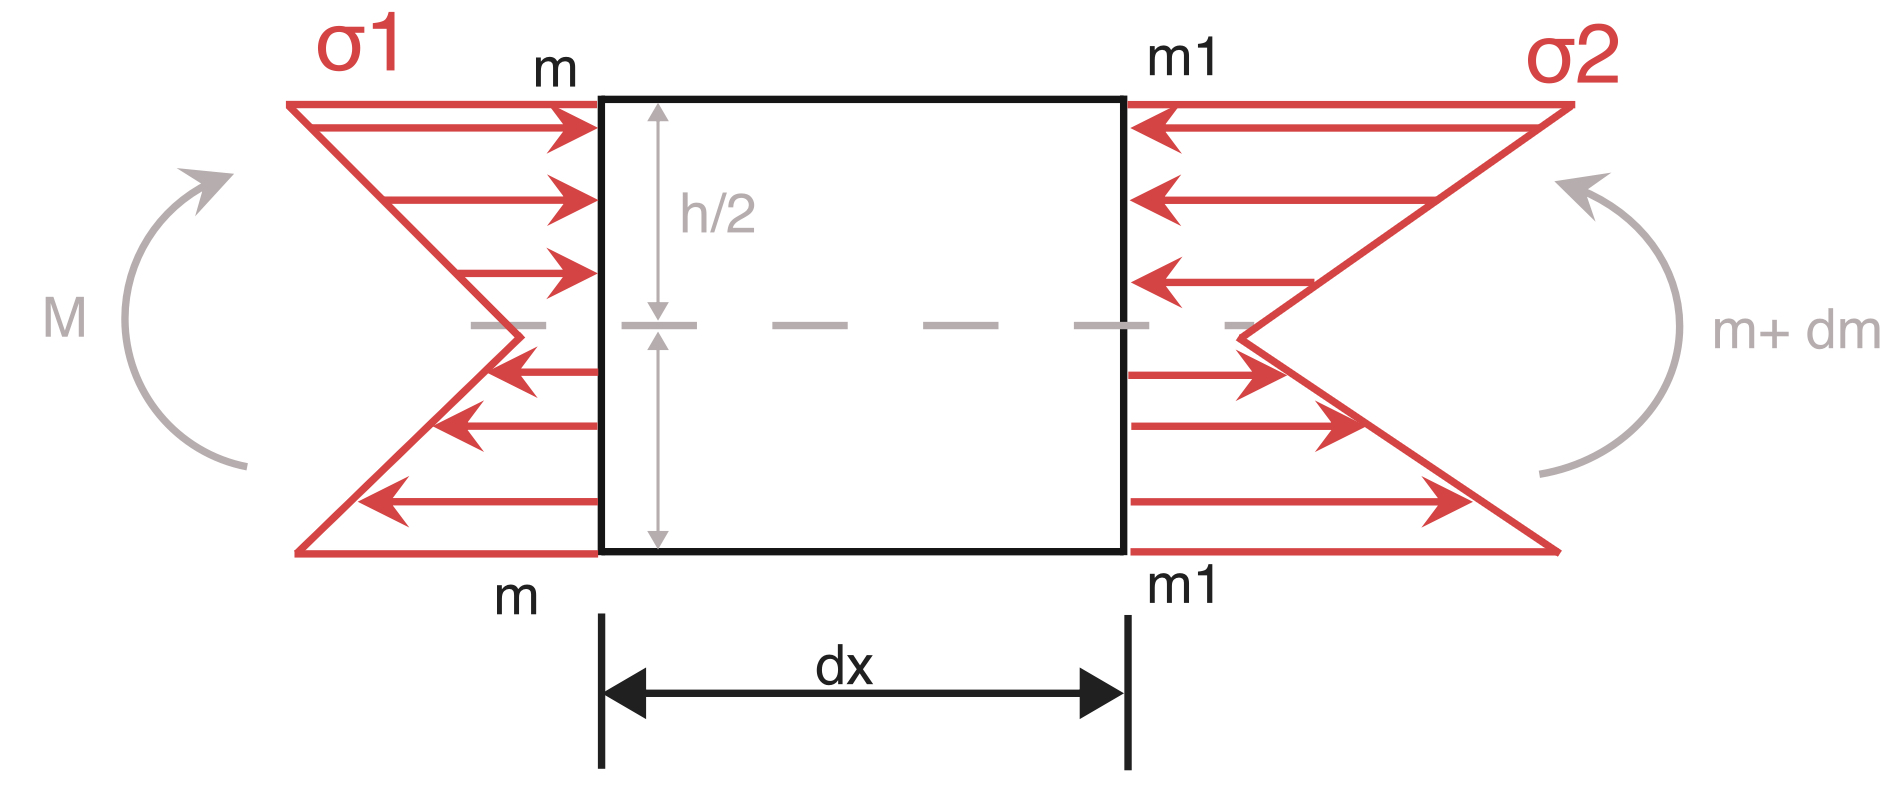
\includegraphics[width=\textwidth]{imgs/IMG_0300.jpeg}
        \caption{Tensões}
        \label{fig:enter-label}
    \end{subfigure}
        \begin{subfigure}[t]{.45\textwidth}
        \centering
        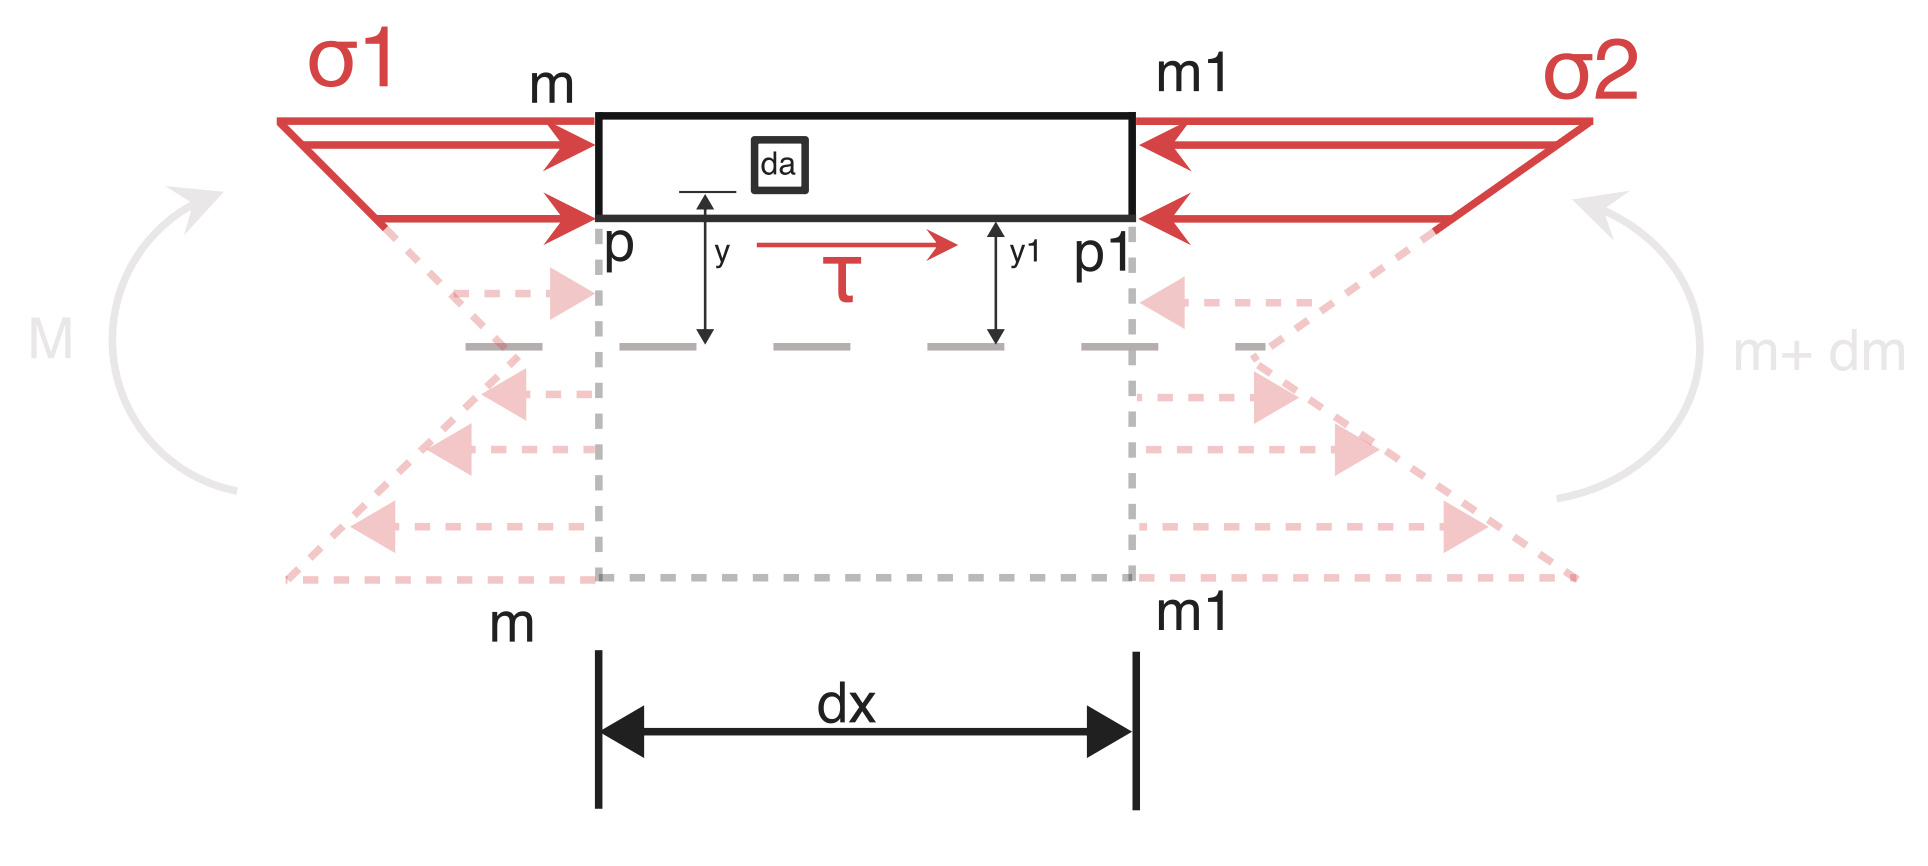
\includegraphics[width=\textwidth]{imgs/IMG_0302.jpeg}
        \caption{Elemento Infinitesimal}
        \label{fig:enter-label}
    \end{subfigure}
\end{figure}

\begin{enumerate}
    \item Nós podemos, primeiramente, dividir a viga em um sub-elemento, definido pelas arestas $\{m,m - m_1,m_1\}$.
    \item  A partir disso, podemos verificar um carregamento não uniforme (i.e de um lado há uma força de cisalhamento e um momento feltor maior do que no outro). 
    \item Através de ferramentas vistas em resmat I, temos que as tenões normais, para o lado esquedro e lado direito são dadas, respectivamente, por:
    \begin{align*}
        \sigma_1 = \frac{-My}{I}, \ \ \sigma_2 = \frac{-(M + dm)y}{I}
    \end{align*}
    \item Isolando um sub-elemento, de área $dA$, definido por $\{m,m - p_1,p_1\}$, que está a uma altura $y$ da linha neutra, somos capazes de calcular as tensões de cisalhamento $\tau$ considerando o equilíbrio na direçao $x$ do subelemento. \textbf{Isso é valido somente se houver uma diferença entre os momentos feltores}.
    \item Aplicando o fato de que tensão nada mais é do que uma força sobre uma área, e utilizando o equilíbrio estático do sub elemento $\{m,m - p_1,p_1\}$, onde se é aplicado as forças devido a $\sigma_1$ (que conhecemos por RESMAT I), $\sigma_2$ (que conhecemos por RESMAT I) e $\tau$ (Desconhecida),é possível determinarmos uma fórmula para $\tau$, sendo essa:
    \begin{align}
        \tau = \frac{VQ}{Ib}, \ \ \ Q = \int y dA = \frac{b}{2}\left(\frac{h^2}{4} - y_1^2\right)
        \label{eq:ten_cis_vigas}
    \end{align}

    \subitem $\circ$ Onde $y_1$ representa a altura, a partir da linha neutra, que estamos calculado a tensão de cisalhamento.
    \subitem $\circ$ Onde $V$ representa o esforço cortate/forçca de cisalhamento.
    \subitem $\circ$ Onde $I$ representa o momento de inércia.
    \subitem $\circ$ Onde $b$ representa a largura da viga.
\end{enumerate}

Teremos, ainda, que a tensão de cisalhamento máxima $\tau_{max}$ ocorre na linha neutra, e possui o valor de:
\begin{align}
    \tau_{max} = \frac{Vh^2}{8I} = \frac{3V}{2A}, \ \ A = bh
\end{align}

Algo importante de ser falado é que, existem outras fórmulas para o calculo da tensão média, mas essas devem ser usadas com cuidado, pois a tensão máxima é $50\%$ maior do que a tensão média.

\subsection{Vigas de Seção Circula}
Para vigas de seção retangular, nós assumimos que as tensões de cisalhamento eram paralelas ao eixo $y$, pois elas eram paralelas ao esforço cortate $V$. 

Isso, entretanto, não pode ser afirmado para vigas de seção circular. Por isso, nós iremos analizar as tensões de cisalhamento que estão ao longo da linha neutra, e não em qualquer posição, pois elas sim são paralelas ao eixo $y$.

\subsubsection{Vigas Maciças}
para vigas maciças, nós podemos podemos ainda utilzar a fórmula \ref{eq:ten_cis_vigas}, sendo que a única coisa que muda é o $Q$ (que é chamado de segundo momento de área da viga) e o $I$ (momento de inércia) pois a geometria mudou, sendo esses:

\begin{minipage}{0.45\textwidth}
    \begin{align}
        I = \frac{\pi r^4}{4}
    \end{align}
\end{minipage}
\begin{minipage}{0.45\textwidth}
    \begin{align}
        Q = A' \bar y \begin{cases}
            A' &=  \frac{\pi r^2}{2} \\
            \bar y &= \frac{4r}{3\pi}
        \end{cases}
    \end{align}
\end{minipage}

\vspace{10px}
Onde teremos que a tensão de cisalhamento máxima é dada por:
\begin{align}
    \tau_{max} = \frac{4V}{3A}
\end{align}

\subsubsection{Vigas Vazadas}
Já para vigas vazadas teremos:

\begin{minipage}{0.45\textwidth}
    \begin{align}
        I = \frac{\pi}{4} (r_2^4 - r_1^4)
    \end{align}
\end{minipage}
\begin{minipage}{0.45\textwidth}
    \begin{align}
        Q = \frac{2}{3}(r_2^3 - r-1^3)
    \end{align}
\end{minipage}

\vspace{10px}
Com a seguinte tensão máxima:
\begin{align}
    \tau_{max} = \frac{4V}{3A}\left(\frac{r_2^2 + r_2r_1 + r-1}{r_2^2 + r_1^2}\right), \ \ \ A = \pi(r_2^2 - r_1^2)
\end{align}

Esse método de calcular para as vigas circulares é uma aproximação, mas possui um erro muito pequeno quando comparado com outros métodos que são mais complexos, por isso é utilizado.

\newpage
\subsection{Vigas com alma e falanges}
\begin{wrapfigure}[13]{r}
    \centering
    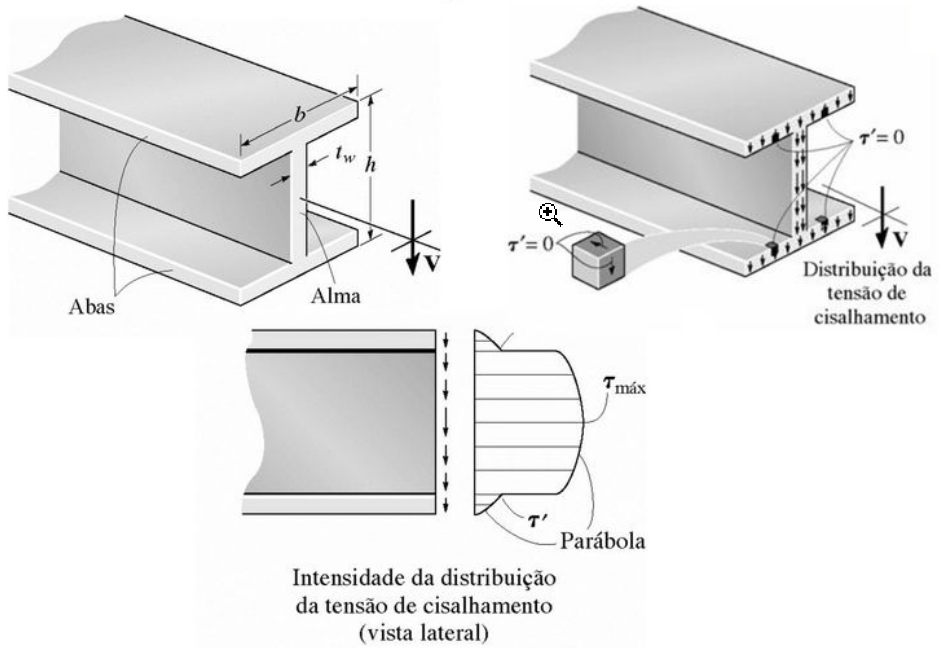
\includegraphics[width=.5\textwidth]{viga_com_alma.png}
    \caption{Viga com Falange e Alma}
    \label{fig:viga_com_alma}
\end{wrapfigure}
Nos casos de vigas com falanges e almas (como exemplificado na imagem ao lado) nós temos que a grande maioria das tensões presentes estão localizadas na alma e são verticais (representam cerca de 90$\%$ a 98$\%$ de todas as tensões).
Tais tensões podem ser obtidas pela mesma fórmula \ref{eq:ten_cis_vigas}.

Nesse caso, teremos o segunda momento de área $Q$ dado por:
\begin{align}
    Q = \frac{b}{8}(h^2 - h_1^2) + \frac{t}{8}(h_1^2 = 4y_1^2)
\end{align}

Onde:
\begin{itemize}
    \item $h \rightarrow$ Altura total da viga
    \item $h_1 \rightarrow$ Altura da alma
    \item $t \rightarrow$ Espessura da alma
    \item $y_1 \rightarrow$ Distância da linha neutra até a linha onde está sendo analisado as tensões de cisalhamento.
\end{itemize}

Já o momento de inércia $I$ é dado por:
\begin{align}
    I = \frac{1}{12}\left(bh^3 - bh_1^3 + th_1^3\right)
\end{align}

Além disso, podemos ver que o perfil de tensão de cisalamento na alma é dado por curva quadrática (como podemos ver pela figura \ref{fig:viga_com_alma}. Temos, então, que os pontos e tensão mínimas e máxima são $y_1 = h_1/2$ e $y_1 = 0$, respectivamente, resultando em:

\begin{minipage}{0.45\textwidth}
    \begin{align}
        \tau_{max} = \frac{V}{8It} (bh^2 - bh_1^2 + th_1^2)
    \end{align}
\end{minipage}
\begin{minipage}{0.45\textwidth}
    \begin{align}
        \tau_{min} = \frac{Vb}{8It} (h^2 - h_1^2)
    \end{align}
\end{minipage}

\vspace{15px}
 Como temos que a grande maioria das tensões de cisalhamento estão na alma, temos que os projetistas calcula uma tensão média através da fórmula abaixo, que está um um range de $10\%$ do máximo (por isso é bastante usado):
 \begin{align}
     \tau_{media} = \frac{V}{th_1}
 \end{align}

 Dévido a essa proximidade ($10\%$) do valor máximo, ele é bastante utilizado por projetistas como aproximação do $\tau_{max}$.
 
 \newpage
 \section{Tensor de Tensões}

 O estado de tensões nada mais é do que uma referência a todas as tensões que estão sendo aplicadas em um ponto, referente a um plano específico. Isso implica que o estado de tensões é depende do plano que está sendo analisado e, como existem infinitos planos que podem passar por um ponto, existem infinitos estados de tensão. 

 Conseguimos, entretanto, calcular todas as tensões (independentes da posição) a partir de 3 vetores de tensão conhecidos associados a três planos perpendiculares entre sí, que chamamos de \textbf{Tensor de Tensões}.

\newpage
\section{Análise de Tensão}

\subsection{Estado Plano}
\subsubsection{Introdução}

 \begin{wrapfigure}[12]{r}
    \centering
    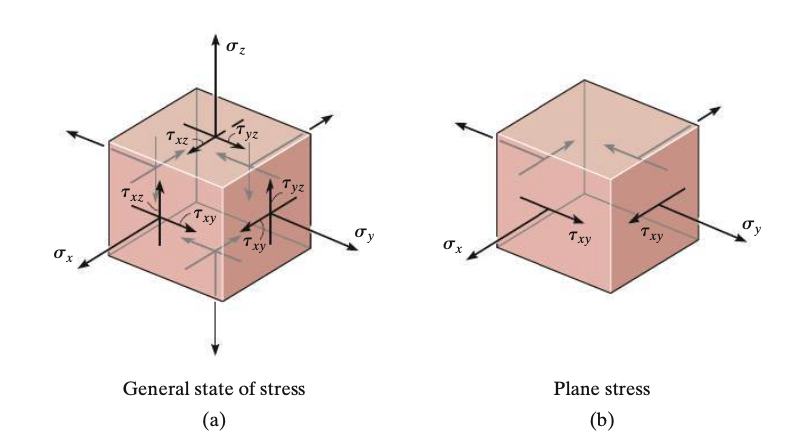
\includegraphics[width=.4\textwidth]{imgs/Estado_plano.png}
    \caption{Simplificação do E. de Tensões}
    \label{fig:simp_estado_tensoes}
\end{wrapfigure}

Vimos que podemos analisar o estado de tensões em um ponto de uma estrutura através do tensor de tensões (um tenso de 3 dimensões). Na maioria das vezes, entretanto, quando estamos lidando com problemas de engenharia nós somos capazes de fazer simplificações tal que somos capazes de analisar o estado de tensões em \textbf{somente um plano}. 


Um exemplo é quando temos um corpo (tri-dimensional e real) não está sofrendo nenhum carregamento em sua superfície. Isso significa que tanto as componentes normais ($\sigma_z$) quanto de cisalhamento ($\tau_{xz}=\tau_{yz} = 0$) da face superior, e por conseguinte todas as componentes simétricas $\tau_{zx}$ e $\tau_{z_y}$, são núlas, resultando em um estado plano de estresse, como podemos ver na imagem ao lado.

Dessa forma, temos que o estado geral de estresse plano é caracterizado através de apenas duas tensões normais ($\sigma_x$ e $\sigma_y$) e somente uma tensão de cisalhamento $\tau_{xy}$. Além disso, é importante ressaltar que \textbf{cada estado de tensão é único para o ponto e o ângulo $\theta$ sob análise}, isso significa que, se quisermos analisar o estado de tensão no mesmo ponto, mas para uma orientação $\theta'$  diferente, precisaremos calcular o novo estado (que veremos mais adiante que será feito através do circulo de Morh).
 

\subsubsection{Círculo de Mohr}
Vimos acima que para um mesmo ponto existem infinitos estados planos de tensão, a depender da orientação. A fim estudarmos a relação entre estado de tensão e orientação (dado pelo ângulo $\theta$), nós usamos o Circulo de Mohr, que é uma ferramenta gráfica derivada a partir das equações de transformação entre planos de estresse.

Como o nome sugere, o círculo de Morh é uma representação gráfico (um círculo), que relaciona a distribuição de tensões (entre tensão normal, no eixo $x$ e cisalhante $y$) em um ponto a depender do ângulo. 

Para sua construção temos que ele possui seu centro e seu raio, respectivamente:

\begin{align}
    X_ = \frac{\sigma_x + \sigma_y}{2}, \ \ R = \sqrt{\left(\frac{\sigma_x - \sigma_y}{2}\right)^2 + \tau^2_{xy}}
    \label{eq:circulo_mohr}
\end{align}

Nós utilizamos esse circulo para calcular, a partir de uma orientação com as tensões conhecidas, os novos valores de tensões de cisalhamento e normais para qualquer nova orientação, pois existe uma relação entre o angulo entre a nova orientação e a orientação original $\theta_{real}$ e o angulo a ser analisado no circulo $\theta_{circ}$, onde $\theta_{circ} = -2\theta_{real}$, isso é, para um angulo $\theta_{real}$ entre a orientação de análise conhecida e a nova face de estudo, nós analisamos no circulo de Mohr um ponto que está a duas vezes $\theta_{real}$, mas no sentido contrário, como podemos ver pela imagem abaixo:


\begin{figure}[h]
    \centering
    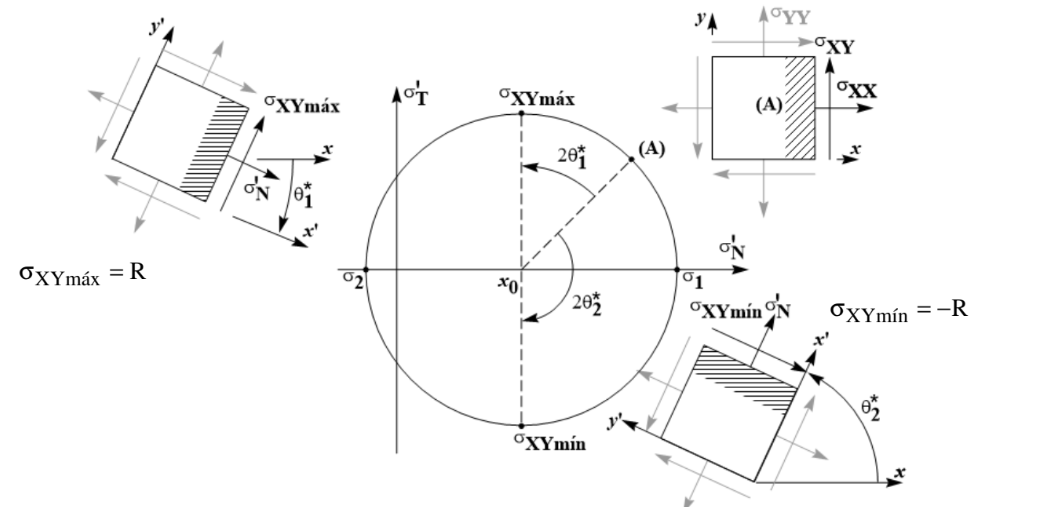
\includegraphics[width=.8\textwidth]{imgs/cir_mohr.png}
\end{figure}

Ser capaz de analisar os novos valores das tensões normais e de cisalhamento é importante pois certo materiais não são capazes de sustentar tensões normais de forma eficiente, o que pode levar a sua fadiga. Por isso denominamos a orientação com o maior valor de tensão normal ($ \sigma_{n_{max}} = X_0 + R$) de \textbf{plano principal}. Além disso temos também os \textbf{Planos de Cisalhamento Máximo} que, como a origem do circulo está sempre no eixo $x$ (eixo das tensões normais), possui o valor máximo de tensão de cisalhamento igual a $R$ (igual ao raio do circulo).

\newpage
Para facilitar a solução de problemas através do circulo de Morh temos o seguinte passo a passo:
\begin{enumerate}
    \item \textbf{Montar Tensor de Tensão}: Como dito anteriormente, somos capazes de ver cada componente da tensão a partir da relação $F/A$ a partir das forças e áreas relacionadas.
    \item \textbf{Calculo de Centro}: Calcular o centro do circulo a partir das tensões normais.
    \item \textbf{Calculo de Raio}: Calcular o raio do circulo.
    \item \textbf{Desenhar o Circulo}: Desenhar com os eixos corretos, com o centro e valores máximos e mínimos corretos.
    \item \textbf{Localizar Ponto Conhecido}: A partir do tensor nós podemos representar a face $x$ (utilizando a primeira linha do tensor) ou a face $y$ (utilizando a segunda linha). A melhor escolha é aquela que facilita encontrar o ângulo alvo de análise.
    \item \textbf{Desenhar Corpo a ser Analisado}: Nós fazemos o circulo a partir de uma posição conhecida (consideramos essa posição $\theta=0$), e é necessário desenhar o corpo na nova posição a ser analisado para facilitar a identificação do ângulo do plano $\theta_{target}$
    \item \textbf{Análise do Circulo}: Analisar o ponto $\theta_{circ} = -2 \theta_{target}$
\end{enumerate}

\newpage
\subsection{Estado Tri-Dimensional}
\subsubsection{Introdução}
 \begin{wrapfigure}[7]{r}
    \centering
    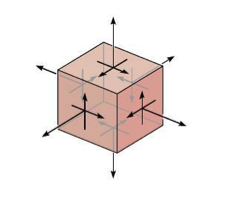
\includegraphics[width=.3\textwidth]{imgs/estado_geral.png}
\end{wrapfigure}
Quando um corpo está sob um estado genérico de tensões tri-dimensional, temos que um elemento de tal corpo sob análise possui uma tensão normal e duas tensões de cisalhamento para cada uma de suas faces, como podemos ver pela imagem ao lado. A partir disso, somos capazes de construir um circulo de Morh para cada uma das suas faces, que se traduz para um circulo de mor para cada "par de coordenada" ($x-y, x-z, y-z$), a fim de representarmos todo o estado de tensão (tri-dimensional) a partir das simplificações e facilidades da análise de estado plano.

\subsubsection{Circulo de Morh - Estado 3D}
Para se construir o circulo de Morh para um estado 3D de tensões, nó temos que fazer exatamente os mesmos passo que foram feitos para o estado plano de tensão, mas um total de 3 vezes, cada uma utilizando um plano como referência. 

Tendo como exemplo o estado de tensão da figura \ref{fig:carregamento_geral}, nós primeiramente iremos analisar o plano $z-y$, posteriormente o plano $z-x$ e por último o plano $y-x$.
\begin{figure}[h]

    \centering
    \begin{subfigure}[t]{.45\textwidth}
        \centering
        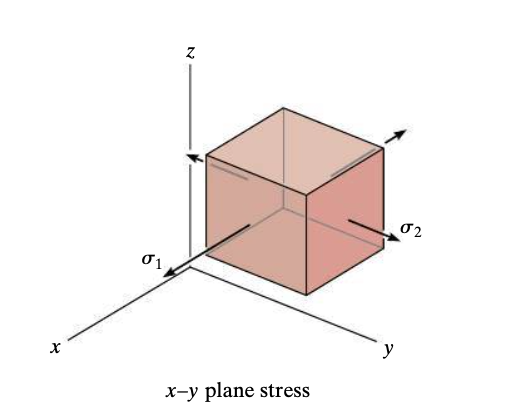
\includegraphics[width=0.6\textwidth]{imgs/exemplo_3d.png}
        \caption{Carregamento 3D}
        \label{fig:carregamento_geral}
    \end{subfigure}
    \begin{subfigure}[t]{0.45\textwidth}
        \centering
        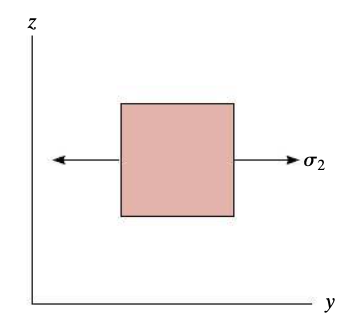
\includegraphics[width=.5\textwidth]{imgs/exemplo_3d_zy.png}
        \caption{Plano $z-y$}
        \label{fig:enter-label}
    \end{subfigure}
        \begin{subfigure}[t]{.45\textwidth}
        \centering
        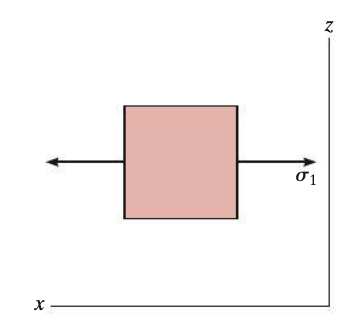
\includegraphics[width=0.5\textwidth]{imgs/exemplo_3d_zx.png}
        \caption{Plano $z-x$}
        \label{fig:enter-label}
    \end{subfigure}
    \begin{subfigure}[t]{.45\textwidth}
        \centering
        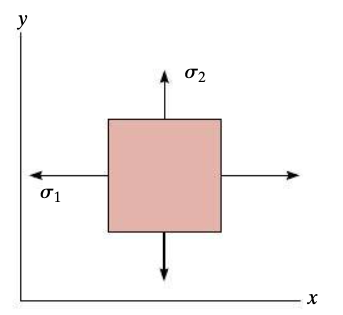
\includegraphics[width=0.5\textwidth]{imgs/exemplo_3d_yx.png}
        \caption{Plano $y-x$}
        \label{fig:enter-label}
    \end{subfigure}
    \caption{Análise - Estado Tri-Dimensional de Tensão}
\end{figure}

\begin{enumerate}
    \item \textbf{Análise do Plano $z-y$}: Ao analizarmos as tensões presentes no plano $z-y$, vemos que há somente a tensão normal $\sigma_2$. Ao aplicarmos as formulas do círculo de Morh (\ref{eq:circulo_mohr}), temos que o primeiro circulo de Mohr terá centro no ponto $X = \sigma_2/2$ e raio de $R = \sigma_2/2$.
    \item \textbf{Análise do Plano $z-x$}: Analogamente à análise feita para o plano $z-y$, no plano $z-x$ temos que há somente uma tensão normal $\sigma_1$ presente, resultando no segundo circulo de Mohr tendo centro em $X = \sigma_1/2$ e raio $R = \sigma_1/2$.
    \item \textbf{Análise do Plano $y-x$}: Analisando, então, o plano $y-x$, podemos ver que há duas tensões normais ($\sigma_1$ e $\sigma_2$), resultando no último circulo de Mohr com centro em $X = (\sigma_1 + \sigma_2)/2$ e um raio de $(\sigma_1 + \sigma_2)/2$.
\end{enumerate}

Resultando em três circulos de Morh, que podem ser sobrepostos, como na figura \ref{fig:morh_circ_3d}.

\newpage
\subsubsection{Tensão Máxima Absoluta de Cisalhamento}

\begin{wrapfigure}[11]{r}
    \centering
    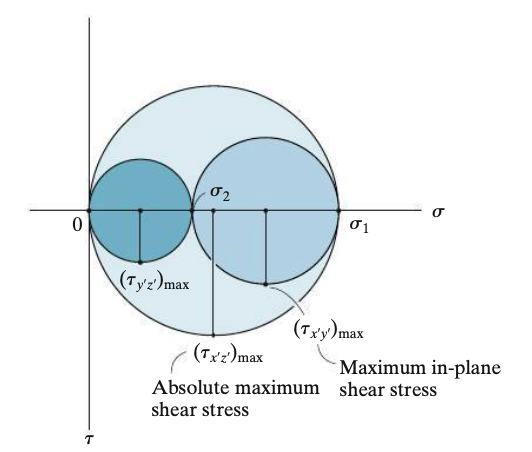
\includegraphics[width=0.4\textwidth]{imgs/circ_mohr_3d.png}
    \caption{Circ. Morh - Estado 3D}
    \label{fig:morh_circ_3d}
\end{wrapfigure}

Assim como no estado puramente plano de tensões, a partir do circulo de Morh nós podemos analisar as tensões de cisalhamento máximas e cada uma das faces do estado tri-dimensional de tensão.

Para os casos onde $sign\{\sigma_1\} = sign\{\sigma_2\}$ temos:
\begin{align}
    \tau_{abs_{max}} = \frac{\sigma_{max}}{2}
\end{align}

Já para os casos onde $sign\{\sigma_1\} \ne sign\{\sigma_2\}$ temos:

\begin{align}
    \tau_{abs_{max}} = \frac{(\sigma_{max} - \sigma_{min})}{2}
\end{align}

\newpage
\section{Carregamentos Combinados}
\subsection{Introdução}
Quando falamos de carregamentos combinados, estamos nos referindo aos casos onde, em um mesmo corpo, estão presentes carregamentos axiais, torcionais, feltores e cisalhantes. 

Iremos falar, mais especificamente, da análise das tensões nos chamados \textbf{Vasos de Pressão de Paredes Finas}, muito utilizados no transporte e armazenamento de fluidos.

\subsection{Vasos de Pressão de Paredes Finas}
Mais comumente cilíndricos ou esféricos, vesos de pressão são usados com bastante frequência em engenharia, seja como reservatórios ou boilers. Para ser considerando de parede fina, entretanto, é necessário que a razão entre o diâmetro interno e a grossura do parede seja $r/t \ge 10$, o que, na grande maioria das vezes, é o caso.

Pelo fato de ser relativamente fina a parede dos vasos de pressão, podemos assumir que não há variação de tensão através da grossura, o que resulta em uma análise bem mais simples das forças atuantes (a partir da análise estática do sistema) e por conseguinte das tensões.

\subsubsection{Vasos Cilíndricos}
Para analisarmos as tensões em vasos cilíndricos, basta analisarmos as condições de equilíbrio estático para o sistema. 

Para um vaso de espessura $t$, raio interno de $r$ e uma pressão $p$, podemos fazer um corte longitudinal (como mostrado na imagem \ref{fig:vaso_c_eixo_x}) e, ao fazermos a análise para equilíbrio estático no eixo $x$, somos capazes de encontrar a pressão circular \footnote{Chamaos de circular por ser tangente ao perfil circular} $\sigma_1$.

\begin{align}
    \sigma_1 = \frac{pr}{t}
\end{align}

Analogamente, através de um corte transversal (figura \ref{fig:vaso_c_eixo_y}) e da análise de equilíbrio no eixo $y$, somos capzes de encontrar a pressão longitudinal $\sigma_2$:
\begin{align}
    \sigma_2 = \frac{pr}{2t}
\end{align}

Onde podemos ver que a tensão circular $\sigma_1$ é o dobro da tensão longitudinal $\sigma_2$. Isso implica que, em caso de falha, ocorrera um "rasgo" paralelo ao eixo do vaso, ao invés dele se romper em dois perpendicularmente ao eixo.
\begin{figure}[h]

    \centering
    \begin{subfigure}[t]{.45\textwidth}
        \centering
        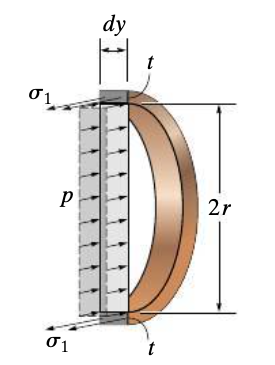
\includegraphics[width=0.6\textwidth]{imgs/vaso_c_1.png}
        \caption{Análise - Eixo $x$}
        \label{fig:vaso_c_eixo_x}
    \end{subfigure}
    \begin{subfigure}[t]{0.45\textwidth}
        \centering
        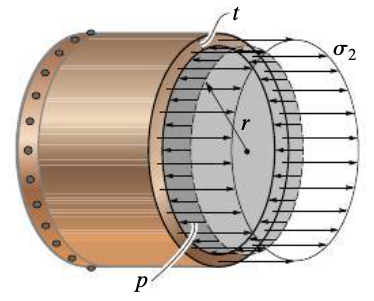
\includegraphics[width=.7\textwidth]{imgs/vaso_c_2.png}
        \caption{Análise - Eixo $y$}
        \label{fig:vaso_c_eixo_y}
    \end{subfigure}
    \caption{Análise de Pressão - Vasos Cilíndricos}
\end{figure}

\subsubsection{Vasos Esféricos}
Analogamente a como foi feito para vasos cilíndricos, nós podemos analisar as condições de equilíbrio estático de seções dos vasos esféricos para determinar as tensões submetidas. 

A principal diferença, entretanto, é que, devido a sua total simetria, é que haverá somente uma tensão longitudinal $\sigma_2$:
\begin{align}
    \sigma_2 = \frac{pr}{2t}
\end{align}

Quando comparamos as tensões presentes em vasos cilíndricos e vasos esféricos, podemos ver que, para uma mesma pressão interna, raio interno e espessura, \textbf{os vasos esféricos possuem uma pressão máxima 50\% menor que vasos cilíndricos}. E é exatamente por esse fato que para o armazenamento de gases (que necessitam de uma pressão muito mais elevada quando comparada com o armazenamento de fluidos), são usados vasos esféricos.
\begin{figure}[h]

    \centering
    \begin{subfigure}[t]{.45\textwidth}
        \centering
        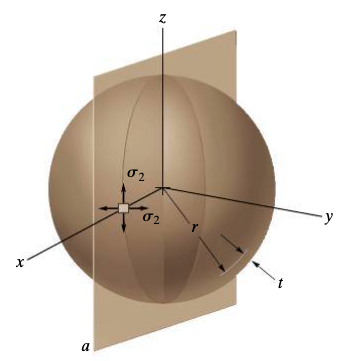
\includegraphics[width=0.8\textwidth]{imgs/vaso_esferico.png}
        \caption{Sistema de Coordenadas}
        \label{fig:vaso_c_eixo_x}
    \end{subfigure}
    \begin{subfigure}[t]{0.45\textwidth}
        \centering
        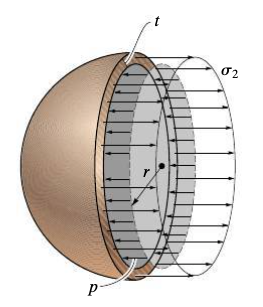
\includegraphics[width=.7\textwidth]{imgs/vaso_esferico_sec.png}
        \caption{Análise - Eixo $y$}
        \label{fig:vaso_c_eixo_y}
    \end{subfigure}
    \caption{Análise de Pressão - Vasos Esféricos}
\end{figure}

\end{document}